\documentclass{article}
\usepackage{graphicx}
\usepackage{caption}
\usepackage{subcaption}
\usepackage{tabularx}
\usepackage{placeins}
\usepackage{amssymb}
\usepackage{array}
\usepackage{todonotes}
\usepackage{biblatex}
\addbibresource{Bibliography/Exercise.bib}

\author{Amalie}
\title{Assignment 2}

\begin{document}
    
\clearpage\maketitle
\thispagestyle{empty}
\newpage
\tableofcontents
\listoffigures
\listoftables

\section{Task 1}

    Find requirements of bachelor thesis. Write a LATEX document explaining your
    findings. Document your sources.
    \newline 

    Da besvarelsen skal være brugbar for os som studerende,har vi valgt at tage udgangspunkt i CPH Business krav til vores kommende bachelor projekt. \cite{softwebsite}

    \subsection*{Krav til Rapporten}
    \begin{itemize}
        \item Da en bachelor svarer til 15 ECTS points, forventes det at den studerende bruger 412,5 time på bachelor projektet.  
            \[ 15 * 27,4 timer = 412,5 timer \]
        \item Det maksimale antal sider afhænger af gruppens størrelse og udregnes således: \(maksantalsider = 40 + 20 * antalstuderende\)
        \item Hvis rapporten er under \(2/3\) af det maksimale antal sider, anses den for at være kort. Der er dog ikke et officelt minimumskrav.  
        \item Rapporten skal skrives på enten dansk eller engelsk.
        \item Rapporten skal indeholde en gennemgående beskrivelse af det udarbejdede projekt, samt evaluering og refleksion over dette.
    \end{itemize}
    \subsection*{Rapportens indhold}
    \begin{enumerate}
        \item Forside (titel, studerendes navne og id, skole og vejleder)
        \item Abstract (ca. 4 linjer og skrives til aller sidst)
        \item Indholdsfortegnelse 
        \item Introduktion
        \begin{itemize}
            \item Motivation
            \item Forventede resultat
            \item Opgaver for at kunne opnå det forventede resultat
            \item Scope
            \item Kort beskrivelse af hvert afsnit efterfølgende
        \end{itemize}
        \item Undersøgelse og redegørelse af teknologier og teori
        \item Krav specfikationer og design
        \item Implementation og udvikling 
        \item Konklusion
        \item Littearturliste og bilag 
        \item Præsentation (eventuelt powerpoint)
    \end{enumerate}

    \subsection{Sources}

\section{Task 2}

    Produce a template (in LATEX, of course) that you can use in your bachelor
    thesis. It should be rich with examples of the following (ie. one of each):

    \subsection{Danish Letters}
    æ ø å

    \subsection{Graphics}

        \begin{figure}[!htp]
            \caption{Caption above image}
            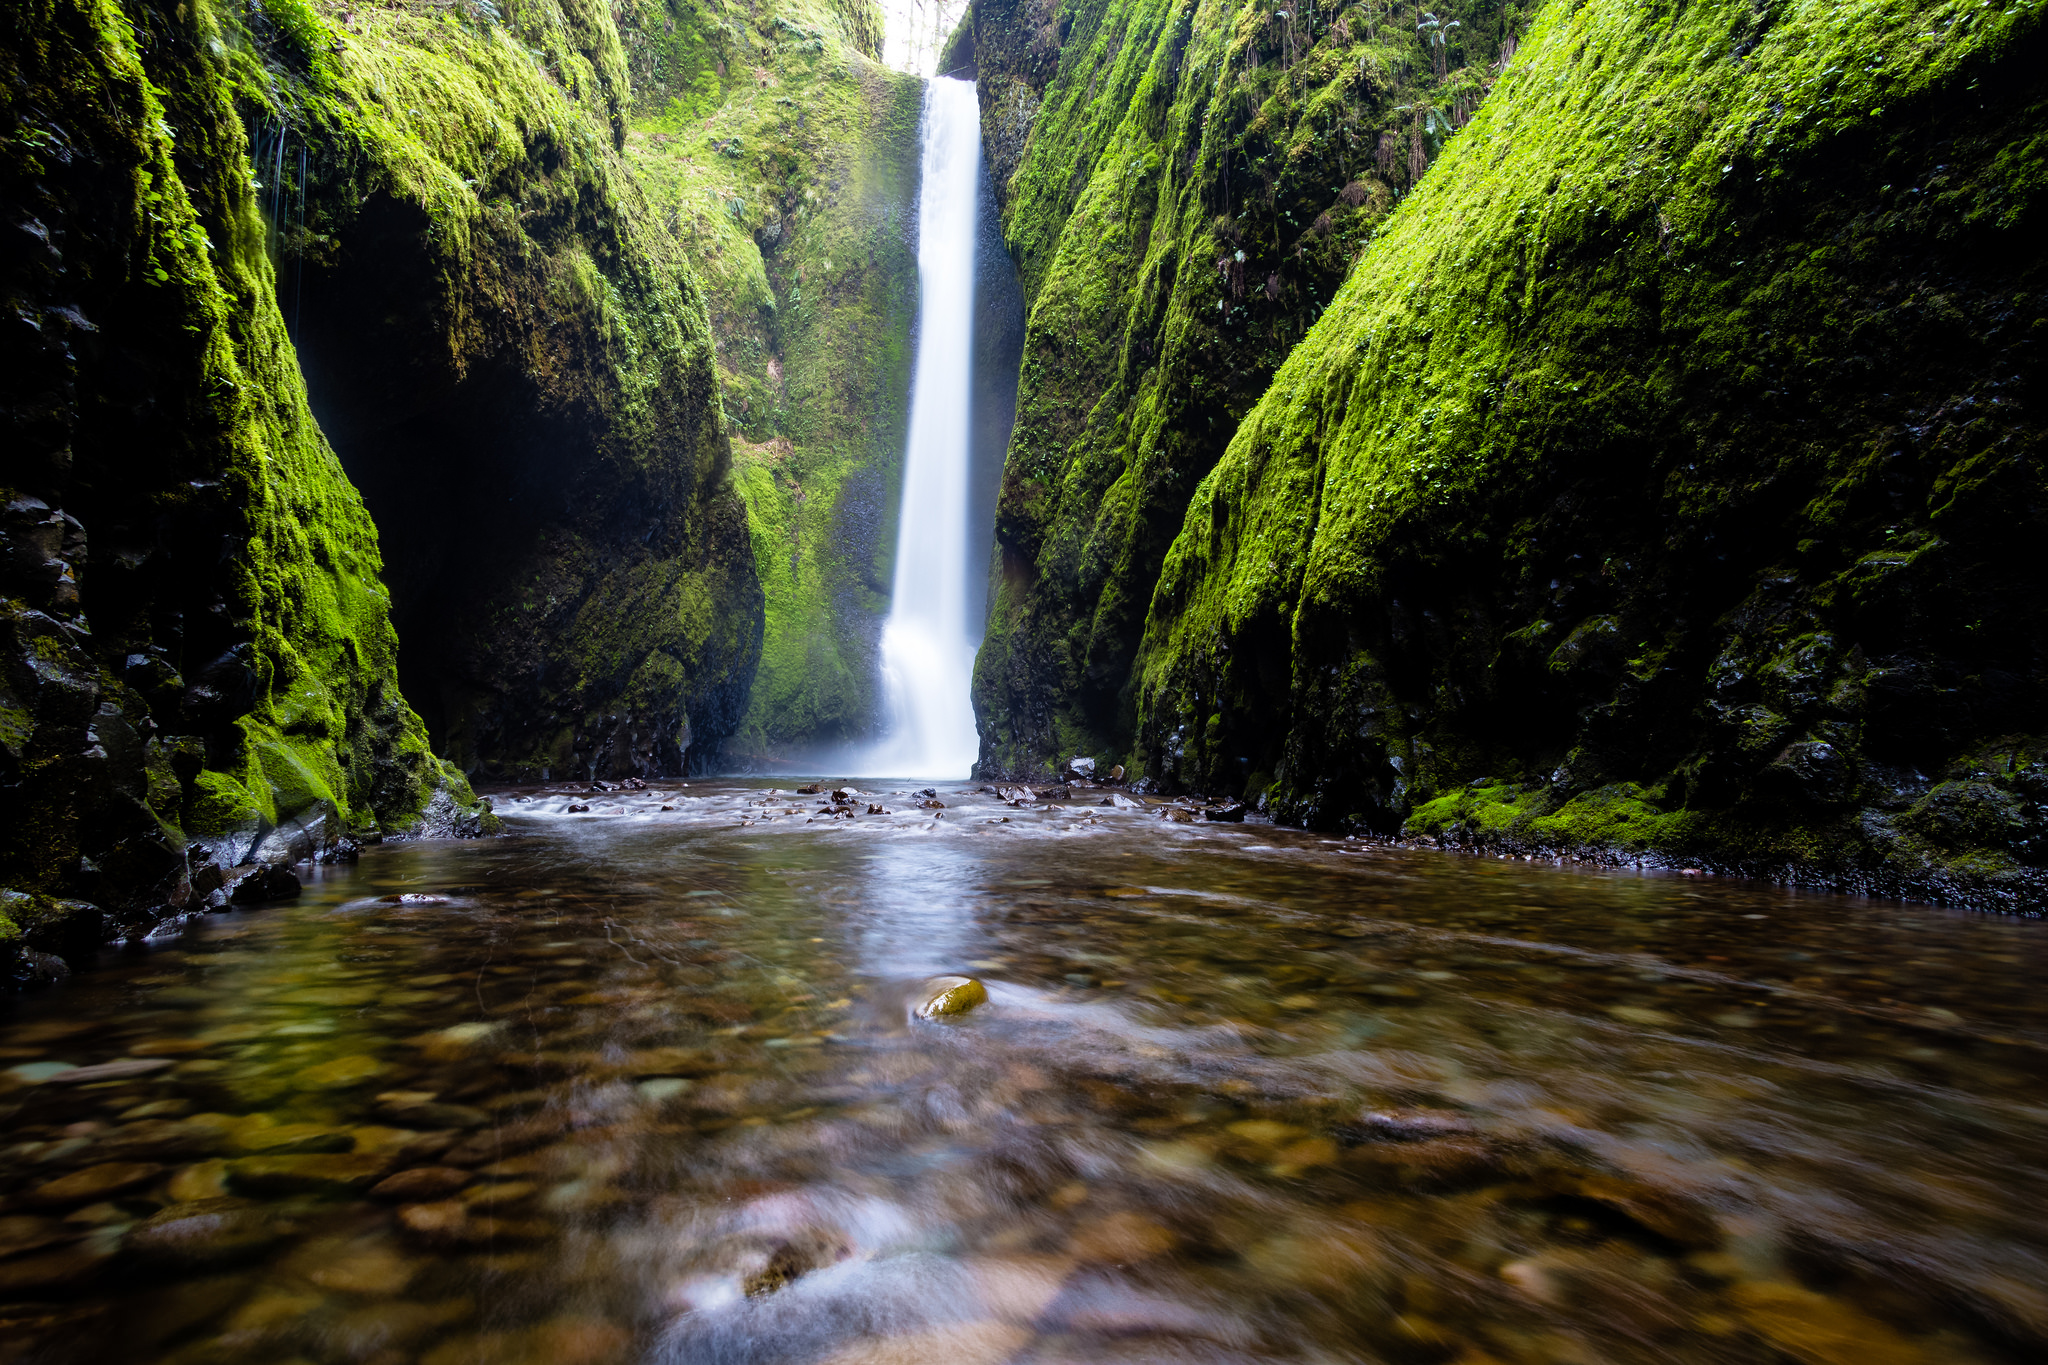
\includegraphics[width=0.5\linewidth]{waterfall.jpg}
            \centering
            \label{fig:waterfall}
        \end{figure}

        \begin{figure}[!htp]
            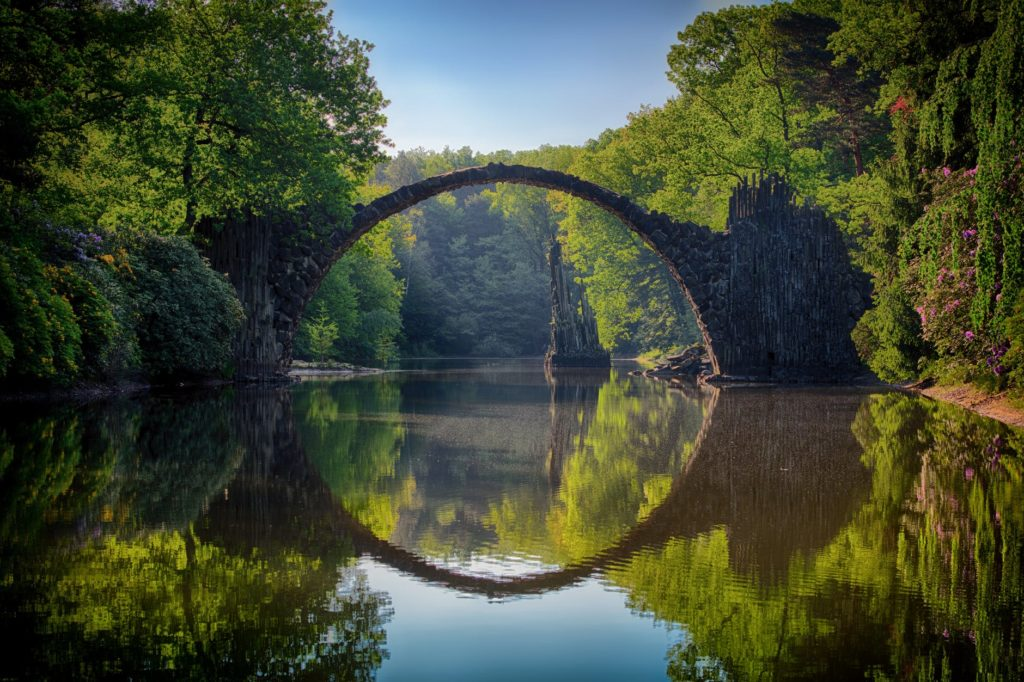
\includegraphics[width=0.5\linewidth]{lake.jpg}
            \centering
            \caption{Caption under image}
            \label{fig:lake}
        \end{figure}
        \FloatBarrier

        \begin{figure}[!htp]
            \begin{subfigure}[b]{0.45\linewidth}
                \centering
                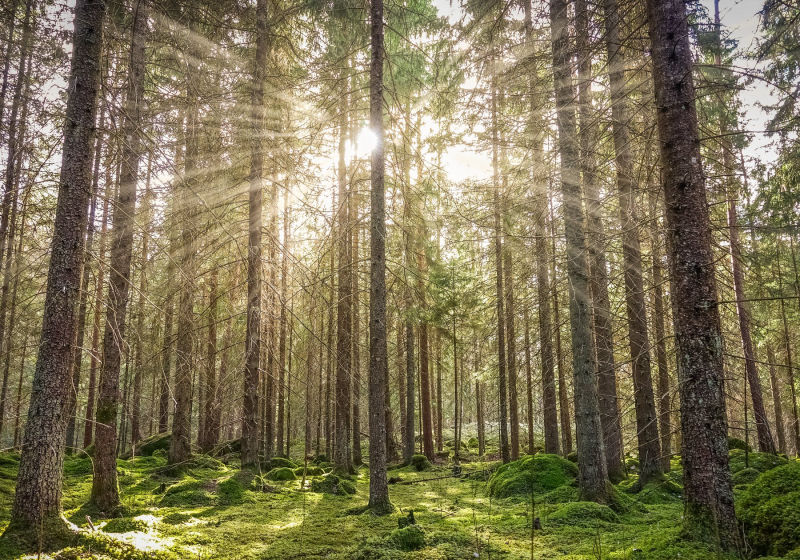
\includegraphics[width=\textwidth]{forest.jpg}
                \caption{This is a forest}
                \label{fig:forest}
            \end{subfigure}
        \hspace{0.5cm}
            \begin{subfigure}[b]{0.45\linewidth}
                \centering
                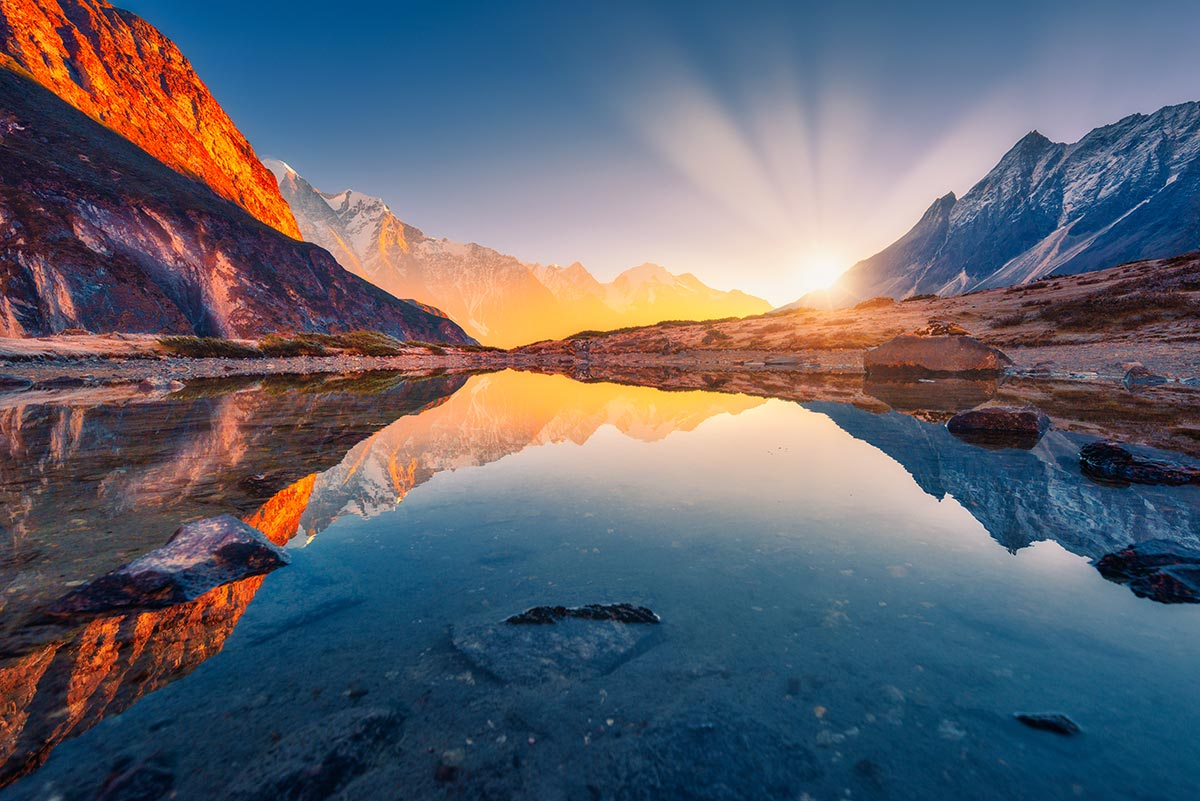
\includegraphics[width=\textwidth]{mountain.jpg}
                \caption{This is a mountain}
                \label{fig:mountain}
            \end{subfigure}
        \caption{This is nature at it's finest}
        \label{fig:nature}
        \end{figure}

    \subsection{References}
    \subsubsection*{To images}
    Figure \ref{fig:mountain} is an image of a mountain. 

    \subsubsection*{To page containing the image}
    An images of a waterfall can be found at page \pageref{fig:waterfall}
    
    \subsubsection{Paragraphs}
        \paragraph{Paragraph}
        This is the first paragraph. This is the first paragraph. This is the first paragraph. This is the first paragraph.
        \subparagraph{Subparagraph}
        This is the second paragraph.

    \subsection{Lists}
        \subsubsection{Bullet points}
            \begin{itemize}
                \item Bullet one
                \item Bullet two
            \end{itemize}

        \subsubsection{Alternativ Bullet}
        \begin{itemize}
            \item[$\checkmark$] Check one
            \item[$\checkmark$] Check two
        \end{itemize}
        
        \subsubsection{Enumerated list}
        \begin{enumerate}
            \item This is another list
            \begin{enumerate}
                \item One 
                \item Two
            \end{enumerate}
            \item And another one
            \begin{enumerate}
                \item Three
                \item Four
            \end{enumerate}
        \end{enumerate}
    
    \subsection{Tables}
        \subsubsection{Table with horizontal alignments in columns}
            \begin{table}[!h]
                \begin{tabularx} {0.5\textwidth} {
                    | >{\raggedright\arraybackslash}X 
                    | >{\centering\arraybackslash}X 
                    | >{\raggedleft\arraybackslash}X | }
                    \hline
                    One & Two & Three \\ \hline
                    Four & Five & Six \\ \hline
                    Seven & Eight & Nine \\ \hline
                \end{tabularx}
                \centering
                \caption{Horizontal alignments left, right and centered}
                \label{table:numbers}
            \end{table}
            
        \subsubsection{Table with a cell spanning multiple columns}
            \begin{table}[!h]
                \begin{tabular}{|c|c|c|}
                    \hline
                    \multicolumn{3}{|c|}{Persons} \\ [1ex]
                    \hline
                    Name & Gender & Age \\ [1ex]
                    \hline
                    Buller & Male & 3 \\ 
                    Buffy & Female & 16 \\ 
                    Bay & Male & 9 \\ 
                    \hline
                \end{tabular}
                \centering
                \caption{Cell spanning multiple columns}
                \label{table:persons}
            \end{table}   
             
            \subsubsection{Reference}
            
            Table \ref{table:numbers} is on page \pageref{table:numbers}
    
                
    \subsection{Code listing - emphasized key words}
    \emph{Java} was originally developed by James Gosling at \emph{Sun Microsystems} (which has since been acquired by \emph{Oracle}) and released in \textbf{1995} as a core component of Sun Microsystems' Java platform. 

    \subsection{Math equations}
        \subsubsection{Inline equations (in text) and equations on separate line}
            Depending on the value of $x$ the equation \( f(x) = \sum_{i=0}^{n} \frac{a_i}{1+x} \) may diverge or converge.
            \[ f(x) = \sum_{i=0}^{n} \frac{a_i}{1+x} \]
    
        \subsubsection{Fractions, summations, products, roots, powers}
            Fraction: 
            \[\frac{1}{4}\]
            Summation: 
            \[\sum\limits_{i=1}^n i^2 = \frac{n(n+1)(2n+1)}{6}\]
            Products:
            \[\prod\limits_{i=1}^n x = x^n\]
            Roots:
            \[ \sqrt{14} \]
            Powers:
            \[ x^n \]
    
    \subsection{Todo notes}
        \todo{This a note}
        \todo{This another note}
    
    \newpage
    \subsection{Bibliography of book, article and internet link}
        An article: \cite{Clear} 
        A book: \cite{latexcompanion}
        A website: \cite{knuthwebsite} 

    \printbibliography
         
    
\end{document}
